\chapter{Our solution} \label{our:solution}
% TODO insert \nopagebreak after \midrule s

In our solution we design an AutoML system for workflow optimization based on
developmental genetic programming. Compared to existing systems it supports 
arbitrary-sized pipelines as well as complex ensemble structures. An overview
of the process is shown in algorithm \ref{alg:genens}.

The input of the
algorithm is the dataset for which we want to find an optimized pipeline, and
configuration of the system. The latter comprises of settings of the
underlying evolutionary algorithm, configuration related to encoding (Tables
\ref{tab03:nodes} and \ref{tab03:methods}, or a user-defined alternative) and
evaluation method along with the metric used for scoring.

The dataset provided to the algorithm must be already preprocessed to some
extent, as no imputation of missing values or string feature encoding is
performed. On the other hand, feature selection and scaling is a part of
the algorithm.

When everything is set up, we run the developmental GP optimization
(line \ref{line:devGP}), which operates with pipelines in a tree-based
representation. The output of this algorithm are individuals which
performed the best on the given datasets. The individuals are decoded into
pipelines (line \ref{line:compile}) and returned as the final output of the
algorithm.

The process of the developmental GP along with the specific tree encoding of
individuals is described in more detail in section \ref{genens:devGP}. 
Evaluation of pipelines and implementation details as well as relation to
scikit-learn (\cite{scikit-learn}) are presented in section \ref{genens:eval}.

\begin{algorithm}
\DontPrintSemicolon 
\caption{Pipeline optimization --- main\label{alg:genens}}
  \KwData{dataset $d$, configuration $c$}
  \KwResult{optimized pipelines}
  \SetKwFunction{Compile}{compile}
  \;
  $individuals \longleftarrow$ run developmental GP on $d$ with $c$ \label{line:devGP} \;
  $pipelines \longleftarrow$ \Compile{$individuals$} \label{line:compile}
  \;\;
  \KwRet{pipelines}
  
\end{algorithm}


\section{Evolutionary optimization of pipelines} \label{genens:devGP}
In this section, we describe the necessary components of the evolutionary algorithm.
The process corresponds to the schema of a general evolutionary algorithm
\ref{alg:EA}. A more detailed schema is presented in algorithm \ref{alg:devgp}.

The input of the algorithm is the population size, maximum number of
generations (which defines the stopping condition), probabilities of a genetic
operator being applied and node arity and tree height limits.

At the beginning, the initial population of individuals, that is, encoded pi\-pe\-li\-nes,
is generated and evaluated (lines \ref{alg:genens:init} and
\ref{alg:genens:genvalid}). If an error occurred during the evaluation of a
pipeline, the corresponding individual is removed from the population. New 
individuals are then generated and evaluated until a valid one is found.

We then run the actual evolutionary optimization (line \ref{alg:evo}).
In every generation, we first perform the parent selection of individuals for
reproduction (line~\ref{alg:parent}). Then, the genetic operators are applied
with well-defined
probabilities one after another (lines \ref{alg:firstop}--\ref{alg:lastop}).
The newly created offspring are evaluated and added
to population of offspring; in case of invalid fitness, we generate a
valid individual instead(lines \ref{alg:offseval}--\ref{alg:offsvalid}).
Finally, the next generation is created by
performing the NSGA-II selection on population of offspring and parents
combined (line \ref{alg:genens:nsga}).

In following sections we describe the components of this particular
evolutionary algorithm in detail. The encoding of pipelines is summarized in
section \ref{sec:encoding} and the initialization procedure is explained in
section \ref{sec:init}. All reproduction operators are presented in section
\ref{sec:repro}. Finally, the selection and fitness are specified in section
\ref{sec:fitsel}.


\begin{algorithm}
{\small

\DontPrintSemicolon 
\caption{Pipeline optimization --- developmental GP \label{alg:devgp}}
  \KwData{population size $k$, maximum number of generations $max\_gen$,
  crossover probability $p_{cx}$,
  mutation probabilities $p_{mut}$, $p_{mut\_node}$, $p_{mut\_args}$,
  height and arity limits $max\_height$ and $max\_arity$ }
  \KwResult{evolved tree individuals}
  \SetNoFillComment
  \SetKwFunction{Cx}{crossover}
  \SetKwFunction{Mut}{mutation}
  \SetKwFunction{Mutnode}{node\_mutation}
  \SetKwFunction{Mutarg}{arg\_mutation}
  \SetKwFunction{Eval}{evaluate}
  \SetKwFunction{Compile}{compile}
  \SetKwFunction{GenValid}{generate\_valid}
  \;
 
  \Fn{\Eval{$ind$}}{ \label{alg:genens:eval}
        $pipe \longleftarrow$ \Compile{$ind$} \;
        $score, time \longleftarrow$ cross-validate $pipe$ on a sample\;
        $ind.fitness \longleftarrow (score, \log\mleft(time\mright))$
  }
  \;
  \Fn{\GenValid{}}{
  		\While{$score$ is not valid}{
           $ind \longleftarrow$ initialize a new individual\;
           $score \longleftarrow$ \Eval{$ind$}
        }
  }  
  \;  
  \tcc{run developmental GP}  
  $P(0) \longleftarrow$ initialize population of GP trees \label{alg:genens:init}
  \;\;
  \tcc{compute fitness of initial population}
  \For{$ind$ in $P(n)$} {  \label{alg:genens:genvalid}
     \Eval{$ind$}\;
     \If{fitness is not valid}{
         \GenValid{$ind$}
     }
  }
  \;
  \tcc{the process of evolution}
  \While{$n < max\_gen$}{ \label{alg:evo}
      
      \;
      \tcc{reproduction} \label{alg:genens:repro}
      \For{$i$ in \Range{$k/2$}} {
         $i_1, i_2 \longleftarrow$ tournament selection from $P(n)$ \label{alg:parent}

         \If{$p_{cx}$} { \label{alg:firstop}
            \Cx{$i_1$, $i_2$} \tcc*[r]{subtree crossover}
         }
         \;
         \If{$p_{mut}$ for $k=1,2$} {
            \Mut{$i_k$} \tcc*[r]{subtree mutation}
         }
         \If{$p_{mut\_node}$ for $k=1,2$} {
            \Mutnode{$i_k$} \tcc*[r]{node mutation}
         }
         \If{$p_{mut\_args}$ for $k=1,2$} {
            \Mutarg{$i_k$} \label{alg:lastop} \tcc*[r]{hyperparameter mutation} 
         }
         
         \;
         \If{\Eval{$i_k$} for $k=1,2$}{ \label{alg:offseval}
             add $i_k$ to offspring population $P_o(n)$
         }
         \Else{
             \GenValid{$i_k$} and add to $P_o(n)$ \label{alg:offsvalid}
         }
      }
      \;
      $P(n+1) \longleftarrow$ NSGA-II selection from $P_o(n)$ and $P(n)$ \label{alg:genens:nsga} \;
  }
  \;
  \KwRet{Pareto front of $P(c)$} 

}
\end{algorithm}


\subsection{Individual encoding} \label{sec:encoding}
\begin{figure}[ht]\centering
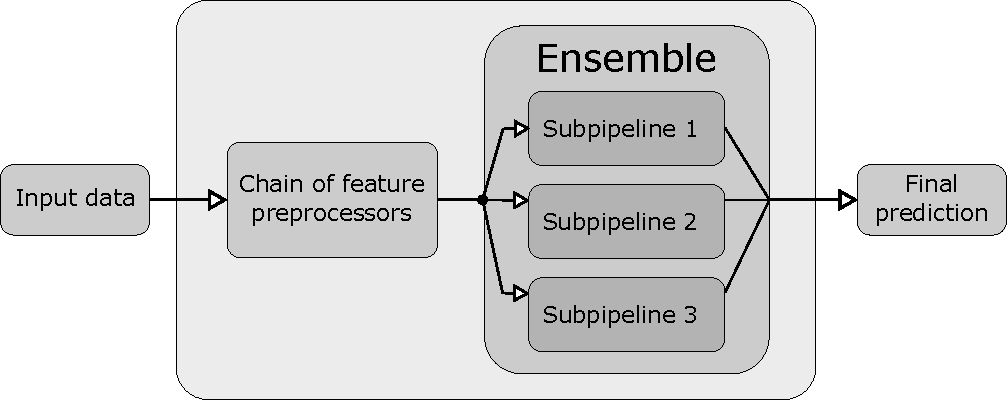
\includegraphics[width=0.7\textwidth]{../img/pipeline-pdfa.pdf}
\caption{Schema of an example pipeline}
\label{pic02:pipeline}
\end{figure}

The encoding is one of the most important parts of this system. The individual
represents a particular ML pipeline, which is composed of a chain of feature
preprocessing methods and of a final estimator. Additionally, we may allow
more complex pipeline steps like ensembles and complex feature
preprocessing methods like stacking or feature union (some of these methods are
described in the book by \cite{Brazdil:2008:MAD:1507541}). In such case, most of the
pipelines become in fact directed acyclic graphs (Figure~\ref{pic02:pipeline}).
Therefore, we cannot directly use the simple tree-based encoding. Instead we
use the developmental GP with cellular encoding described
in section~\ref{devGP}.

In our case, the embryo is an empty pipeline. To create a complex pipeline, we
modify it by inserting steps into it.

\begin{figure}[ht]\centering
    \subfloat[Tree encoding]{{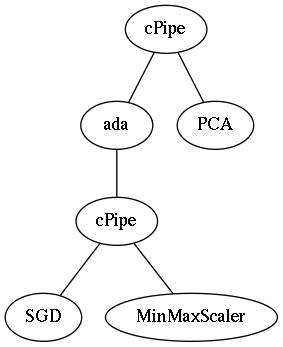
\includegraphics[width=0.25\textwidth]{../img/ada.png} }}%
    \qquad
    \subfloat[Encoded pipeline]{{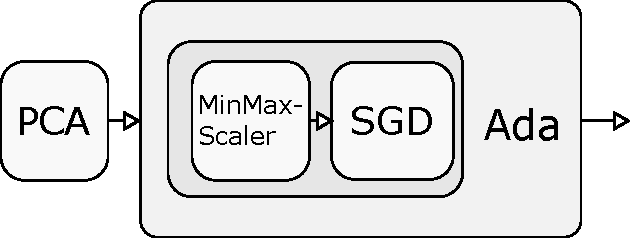
\includegraphics[width=0.5\textwidth]{../img/ada-pdfa.pdf} }}%
    \caption[An example pipeline encoded into a tree individual]{
    An example pipeline encoded into a tree individual. The word \emph{cPipe}
    stands for our pipeline representation, other acronyms refer to
    corresponding ML methods --- the AdaBoostClassifier ensemble method,
    SGD classifier and preprocessing methods PCA and MinMaxScaler.
    }%
    \label{pic:pipeencoding}%
\end{figure}

The process can be demonstrated on Figure
\ref{pic:pipeencoding}. The root of the tree represents the embryo which will
be modified by subsequent operations. In this case, the left subtree modifies
the ensemble structure whereas the right subtree modifies the feature
preprocessor chain. The pipeline contains only one preprocessor, hence the
right subtree is terminated by the corresponding node, PCA in this case. The
left child can be
either an ensemble or a simple method. Here it is the AdaBoost ensemble which
has one base classifier. The subestimator is again a pipeline, which is composed
of a MinMaxScaler and Stochastic gradient descent classifier. The specific
hyperparameters of every pipeline step are stored aside the nodes and are not
depicted in the figures.

\label{sec:decoding}
Table \ref{tab03:nodes} lists all nodes used in the current implementation of
our system. There are several nodes that represent structure altering
operations. The most common nodes are \emph{cPipe} and \emph{cPred}, which
create a pipeline in the model. The pipeline is composed from an estimator
and, in case of \emph{cPipe}, of a feature preprocessor chain. The estimator
may be another pipeline or a single base estimator.

The nodes \emph{cFeatSelect}, \emph{cScale} and \emph{cData} all create the feature
preprocessor chain. The first node creates a chain that contains only a
feature selection method, the second creates a chain with a scaling method
and the last creates a chain with both types of preprocessors. This way, the
methods may be logically ordered one after another. The last node which
operates with preprocessing methods is \emph{dUnion}. It inserts a feature union
into the preprocessor chain --- a method that takes several feature
preprocessing methods and combines the outputs into a final output.

Lastly, we define a specific node for every ensemble, preprocessing and
classifier method which is present in \ref{tab03:methods}. The purpose of
these methods is to define which particular method should be inserted into
a pipeline.

In order to produce reasonable pipelines (i.e. with correct logical ordering of
methods), we use the strongly typed genetic programming.
This means that a node has a well-defined input and output type.
Formally, the input type of is defined as a Cartesian product of types,
whereas the output type is a single type; terminals have only the output type
specified. Output types of
child nodes must match the input type of parent node. The list of nodes
is extensible,
it is possible to add a definition of similar nodes, e.g. a different ensemble
flavour like stacking. The nodes that are specific for a given estimator
correspond to the list of methods in section \ref{tab03:methods}. To decode
the pipeline, the tree is traversed from root to leaves while applying the
operations associated with the nodes.

\begin{table}[ht]

\centering
\caption{Nodes representing modifying operations}\label{tab03:nodes}
\begin{tabular}{l c c p{0.38\textwidth}}
\toprule
\mc{\textbf{Node}\textsuperscript{1}} & \mc{\textbf{In type}\textsuperscript{2}} &
\mc{\textbf{Out type}\textsuperscript{3}} & \mc{\textbf{Operation}} \\
\midrule
cPipe       & ens $\times$ data      & out & Create pipeline with a preprocessor chain and a predictor \\
cPred       & ens                    & out  & Create pipeline only with a predictor \\
cData       & featsel $\times$ scale & data & Create preprocessor chain with feature selector and scaler \\
cFeatSelect & featsel                & data & Create preprocessor chain only with a feature selector \\
cScale      & scale                  & data & Create preprocessor chain only with a scaler \\
dUnion      & $\mbox{data}^n$        & data & Create feature union in the preprocessor chain \\
\textit{ensemble} & $\mbox{out}^n$          & ens  & Insert ensemble \\
\textit{classifier} & $\emptyset$    & out  & Insert classifier \\
\textit{selector} & $\emptyset$      & featsel  & Insert feature selector \\
\textit{scaler} & $\emptyset$        &  scale  & Insert scaler \\
\bottomrule

\multicolumn{4}{l}{\footnotesize
\textsuperscript{1}\textit{There is one specific node per ensemble, classifier
and preprocessor present}} \\

\multicolumn{4}{l}{\footnotesize
\textsuperscript{2}\textit{Variable arity is allowed (i.e. $n \in [1, max\_arity])$}} \\

\multicolumn{4}{l}{\footnotesize
\textsuperscript{3}\textit{In the last level classifier and preprocessing
can have output type $ens$ and $data$ resp.}} 

\end{tabular}

\end{table}

\subsection{Initialization} \label{sec:init}
To initialize an individual, we use a modified grow method (the original algorithm
is described in section \ref{sec:gp:init}). For the initialization process, we
define two sets of nodes. The first ($S_{grow}$) is a set of functions and terminals and is used
in the growing phase, that is, until the height limit is reached. The second set ($S_{term}$)
contains all terminals contained in the first set, and also some additional
terminals --- copies of all classifier nodes, but of output type `ens', and copies
of all preprocessors, but instead of type `data'. The reason of this is that if
there is a cPipe, cPred or dUnion node (Table \ref{tab03:nodes}) in the penultimate level of the tree, there
is no terminal to terminate with in the first set. Thus, the second set is defined
as to be able to finish the initialization properly.

Algorithm \ref{alg:ourgrow} shows the process in detail. Along with the two sets it
takes as it input the height and arity limits and the dictionary of method hyperparameters
associated with the nodes.
First, we determine the height of the tree as a random number between 1 and
$max\_height$, which is the hyperparameter of our system
(line \ref{alg:ourgrow:height}). If the selected height is one, we directly return
a random classifier from $S_{term}$. Otherwise, we insert one of the pipeline
creating operations into the tree (line \ref{alg:ourgrow:root}).

The tree is then grown from root, choosing nodes from $S_{grow}$ or $S_{term}$
respectively. When inserting a node, we first choose a function which has any argument
without a child associated with it. To preserve the type consistency, we randomly
select a node whose output type matches the type of this argument. Also, we choose
its hyperparameters and, if it is a function, we define its arity (this is
described in section \ref{sec:fitsel}). Finally, the node can be inserted as a child
of the function into the tree
(lines \ref{alg:ourgrow:process}--\ref{alg:ourgrow:processend}). This process ends
as soon as all functions have a child for every argument. The output of the algorithm
is the generated individual.

As terminals are inserted in the growing phase as well, the tree may become
smaller than the height limit. However, if the tree were built using the full
method, it would introduce a lot of feature preprocessing methods for taller
trees.

\begin{algorithm}[t]
\DontPrintSemicolon 
\caption{Modified grow method for individual initialization\label{alg:ourgrow}}
  \KwData{maximum height \emph{max\_height}, maximum arity $max\_arity$, sets of nodes
  $S_{grow}$ and $S_{term}$, hyperparameter dictionary $H$}
  \KwResult{generated individual}
  \SetKwFunction{Arity}{choose\_arity}
  \SetKwFunction{HParams}{choose\_hyperparams}
  \;
  $h \longleftarrow$ randomly select tree height from interval $[1, max\_height]$ \label{alg:ourgrow:height}
  \;  
  \If{$h > 1$}{\label{alg:ourgrow:root}
     set $cPipe$ or $cPred$ as the root of $ind$
  }  
  \Else{
      \KwRet{a random classifier from $S_{term}$}
  }
  
  \;
  \While{$ind$ has a function with a child missing}{ \label{alg:ourgrow:process}
      $f \longleftarrow$ a parent node which can accept a child\;
      $t_f \longleftarrow$ argument input type of $f$\;
      $h_{node} \longleftarrow$ height at which the node is inserted
      \;\;
      \If{$h_{node} < h$}{
      $S \longleftarrow S_{grow}$
      }
      \Else{
      $S \longleftarrow S_{term}$
      }
      $node \longleftarrow$ randomly choose a node from $S$ with output type $t_f$\;
      $node.arity \longleftarrow$ \Arity{$node$, $max\_arity$}\;
      $node.hyperparams \longleftarrow$ \HParams{$node$, $H$}\;\;
      
      add the child $node$ as an argument of $f$ \label{alg:ourgrow:processend}
  }
  \KwRet{$ind$}
  
\end{algorithm}

\paragraph{Weighted selection}
During the node selection, we use weights to manage the probability of a node
to be chosen. The motivation is that some nodes represent lightweight methods
which have a short execution time, whereas some nodes slow down the evaluation
process, especially when present multiple times in the tree.

The process is as follows: every node is assigned to a group and each group has
a well defined weight. When selecting a particular node with output type $out$, we 
first determine all groups $G$ which correspond to any node with output type
$out$. Then we select a group $g$ from $G$ by a weighted random choice.
Finally, the node is selected by a simple random choice from $g$.

\paragraph{Variable arity}
Some nodes, e.g. ensemble nodes, may have a \emph{variable arity}.
For example, a voting may have two base estimators or many more, but the
actual model combination method remains the same. Therefore, it is for convenience
represented by a single node type.

The input type of a node is a Cartesian product of its argument types. If we allow
variable arity of each type, the input type is instead defined as
$$t = \prod_{i=1}^{n}t_i^{k_i},$$
where $t_i$ is a specific type, $k_i$ is its arity and $\forall i=1\ldots n - 1, t_i \neq t_{i+1}$.
The representation is defined in a general way as to allow ensembles with groups
of arguments. The ensemble methods used in this work (Table \ref{tab03:nodes})
are all relatively simple, but in future extensions more complex cases may be added.

The actual arity is determined just when the node is about to be inserted
into the tree. The range of possible arities is specified by an interval which may or may not have
an upper bound. If the upper bound is not provided, the values are limited by
a global arity limit ($max\_arity$ in algorithm \ref{alg:ourgrow}) to avoid bloat
of the trees.

\paragraph{Method hyperparameters}
Every node has a list of possible values per hyperparameter associated with
it. During initialization, the actual values are randomly selected from every list.
The validity is not verified in this phase, instead it is handled in the
evaluation phase (section \ref{genens:eval}).

\subsection{Genetic operators} \label{sec:repro}
In our system, we use one type of crossover and three different types of
mutation. The crossover is the standard strongly typed subtree-swap operation,
as described in section \ref{treeops}. The first mutation type is the \emph{subtree
mutation}, which is used to replace whole parts of the pipeline with new structures.
The other two mutation types are more conservative: the \emph{point mutation} replaces
a random node of the tree with a new one, while the \emph{node argument mutation} randomly
changes a hyperparameter of a node.
The mutation operators will be described in more detail in the following paragraphs.

\paragraph{Subtree mutation}
This mutation type is in the most `aggressive' mutation type in this system, as
it greatly alters the structure of a pipeline. As defined in section \ref{treeops},
in subtree mutation a chosen subtree is
replaced with a randomly generated tree. In our implementation we moreover
limit the height of the generated tree. For height $h$ of the subtree, the
height of the newly generated tree must be between $[1, h + \epsilon]$ for a
small value of $\epsilon$. This way we ensure that for small subtrees the new
subtree may be slightly higher and for big subtrees the overall height should
not increase too much. In other words, we try to minimize the bloat induced by
this operation.

\paragraph{Point mutation}
The point mutation enables to change only one step of the pipeline while preserving
the overall structure. In this mutation, a randomly chosen node is replaced with a
new node. Both output and input types must match. Moreover, if the new node
supports variable arity, we must compare the subtypes one by one, as depicted in
\ref{alg:arities}. For this type of mutation, any lower bound of any arity must
be greater than zero.


\begin{algorithm}[t]
\DontPrintSemicolon 
\caption{Input type arity comparation\label{alg:arities}}
  \KwData{type $t$ with fixed arities, type $t'$ with variable arities}
  \KwResult{true if $t$ can be equal to $t'$}
  \;
  \If{the number of subtypes of $t$ and $t'$ differs}{
  \KwRet{false}
  }\;
  
  \For{i in \Range{n}}{
     \If{arity of $t_i$ is not in the arity interval of $t_i'$}{
        \KwRet{false}\;
     }
  }
  \KwRet{true}
\end{algorithm}

\paragraph{Node argument mutation}
Mutates a hyperparameter of a random node --- chooses a new value from the list
of possible values. This method has many possible extensions which are more
described in section \ref{future} (future work).

\subsection{Fitness and selection} \label{sec:fitsel}
To compute the fitness, the individuals are decoded into scikit-learn 
pipelines as described in section \ref{sec:decoding} (individual encoding).
The specific machine learning methods which are used in the pipelines along
with evaluation details are listed in the following section.

The fitness has two objectives~---~evaluation score and logarithmized
evaluation time. The enviromental selection is done via the NSGA-II operator
(described in section \ref{nsgaii}), and the 
parent selection is a tournament selection based on individual dominance and 
crowding distance. This approach allows us to prefer simpler yet
well-performing pipelines, as complex ensemble methods are typically
time-consuming. 

It may happen that some pipeline fails to run, for example due to an
unsupported hyperparameter combination. In that case, the individual is
discarded and a new one is generated. If the next individual is not valid
either, the process is repeated until a valid individual is generated.

\section{Evaluation and performance estimation} \label{genens:eval}
In this section we elaborate on the evaluation process. First we present the
pipelines and used methods in more detail. Then we present the evaluation and
a performance estimation method which was used to decrease the running time.

\subsection{Used machine learning methods} \label{tab03:methods}
We use the scikit-learn implementation of pipelines. An arbitrary pipeline
consists of multiple transformer steps and one predictor step, which is either
an ensemble or a base-learner. Any machine learning method that complies to the
scikit-learn API can act as a pipeline step \citep{sklearn_api}. Regression is
supported by the system as well, but in this work we focus only on
classification problems. Tables \ref{tab:clf}, \ref{tab:prepro} and
\ref{tab:ens} show all machine learning methods present in the default
configuration. Every method has a list of hyperparameter values associated
with it. These are optimized during the process of evolution;
if a hyperparameter is not present, it will be always set to its default value.
The list has been created by slightly extending the hyperparameter list 
used by \cite{Kren2017AutomaticCO} in the AutoML system mentioned in
section \ref{CASH}. 

{\footnotesize
\begin{longtable}{l l}
\caption{Used classifiers with hyperparameters} \label{tab:clf} \\

\toprule
\multicolumn{2}{c}{\textbf{KNeighborsClassifier}} \\*
\midrule

n\_neighbors & [1, 2, 5] \\
algorithm & ['auto', 'ball\_tree', 'kd\_tree', 'brute'] \\

\midrule
\multicolumn{2}{c}{\textbf{LinearSVC}} \\*
\midrule

loss & [hinge,squared\_hinge] \\
penalty & [l1,l2] \\
C & [0.1,0.5,1.0,2,5,10,15] \\
tol & [0.0001,0.001,0.01] \\

\midrule
\multicolumn{2}{c}{\textbf{SVC}} \\*
\midrule

C & [0.1,0.5,1.0,2,5,10,15] \\
gamma & [scale,0.0001,0.001,0.01,0.1,0.5] \\
tol & [0.0001,0.001,0.01] \\

\midrule
\multicolumn{2}{c}{\textbf{LogisticRegression}} \\*
\midrule

penalty & [l1,l2] \\
C & [0.1,0.5,1.0,2,5,10,15] \\
tol & [0.0001,0.001,0.01] \\
solver & [newton-cg,lbfgs,liblinear,sag,saga] \\

\midrule
\multicolumn{2}{c}{\textbf{Perceptron}} \\*
\midrule

penalty & [None,l2,l1,elasticnet] \\
n\_iter & [1,2,5,10,100] \\
alpha & [0.0001,0.001,0.01] \\

\midrule
\multicolumn{2}{c}{\textbf{SGDClassifier}} \\*
\midrule

penalty & [none,l2,l1,elasticnet] \\
loss & [hinge,log,modified\_huber,squared\_hinge,perceptron] \\
max\_iter & [10,100,200] \\
tol & [0.0001,0.001,0.01] \\
alpha & [0.0001,0.001,0.01] \\
l1\_ratio & [0,0.15,0.5,1] \\
epsilon & [0.01,0.05,0.1,0.5] \\
learning\_rate & [constant,optimal] \\
eta0 & [0.01,0.1,0.5] \\
power\_t & [0.1,0.5,1,2] \\

\midrule
\multicolumn{2}{c}{\textbf{PassiveAggressiveClassifier}} \\*
\midrule

loss & [hinge,squared\_hinge] \\
C & [0.1,0.5,1.0,2,5,10,15] \\

\midrule
\multicolumn{2}{c}{\textbf{LinearDiscriminantAnalysis}} \\*
\midrule

solver & [lsqr,eigen] \\
shrinkage & [None,auto,0.1,0.5,1.0] \\\noalign{\penalty-5000}

\midrule
\multicolumn{2}{c}{\textbf{QuadraticDiscriminantAnalysis}} \\*
\midrule

reg\_param & [0.0,0.1,0.5,1] \\
tol & [0.0001,0.001,0.01] \\

\midrule
\multicolumn{2}{c}{\textbf{MLPClassifier}} \\*
\midrule

activation & [identity,logistic,relu] \\
solver & [lbfgs,sgd,adam] \\
alpha & [0.0001,0.001,0.01] \\
learning\_rate & [constant,invscaling,adaptive] \\
tol & [0.0001,0.001,0.01] \\
max\_iter & [10,100,200] \\
learning\_rate\_init & [0.0001,0.001,0.01] \\
power\_t & [0.1,0.5,1,2] \\
momentum & [0.1,0.5,0.9] \\
hidden\_layer\_sizes & [(100,),(50,),(20,),(10,)] \\

\midrule
\multicolumn{2}{c}{\textbf{DecisionTreeClassifier}} \\*
\midrule

criterion & [gini,entropy] \\
max\_features & [0.05,0.1,0.25,0.5,0.75,1] \\
max\_depth & [1,2,5,10,15,25,50,100] \\
min\_samples\_split & [2,5,10,20] \\
min\_samples\_leaf & [1,2,5,10,20] \\

\midrule
\multicolumn{2}{c}{\textbf{GaussianNB}} \\*
\midrule
\multicolumn{2}{c}{\textit{-}} \\

\midrule
\multicolumn{2}{c}{\textbf{GradientBoostingClassifier}} \\*
\midrule

loss & [deviance,exponential] \\
n\_estimators & [20,50,100,200] \\
subsample & [0.3,0.5,0.75,1.0] \\


\midrule
\multicolumn{2}{c}{\textbf{RandomForestClassifier}} \\*
\midrule

n\_estimators & [10,50,100,150,200] \\


\midrule
\multicolumn{2}{c}{\textbf{ExtraTreesClassifier}} \\*
\midrule

n\_estimators & [10,50,100,150,200] \\


\bottomrule

\end{longtable}
}

{\footnotesize
\begin{longtable}{l l}

\caption{Used preprocessors with hyperparameters} \label{tab:prepro} \\

\midrule
\multicolumn{2}{c}{\textbf{NMF}} \\*
\midrule

feat\_frac & [0.01,0.05,0.1,0.25,0.5,0.75,1] \\
solver & [cd,mu] \\

\midrule
\multicolumn{2}{c}{\textbf{FactorAnalysis}} \\*
\midrule

feat\_frac & [0.01,0.05,0.1,0.25,0.5,0.75,1] \\

\midrule
\multicolumn{2}{c}{\textbf{FastICA}} \\*
\midrule

feat\_frac & [0.01,0.05,0.1,0.25,0.5,0.75,1] \\

\midrule
\multicolumn{2}{c}{\textbf{PCA}} \\*
\midrule

feat\_frac & [0.01,0.05,0.1,0.25,0.5,0.75,1] \\
whiten & [False,True] \\

\midrule
\multicolumn{2}{c}{\textbf{SelectKBest}} \\*
\midrule

feat\_frac & [0.01,0.05,0.1,0.25,0.5,0.75,1] \\
score\_func & [feature\_selection.chi2,feature\_selection.f\_classif] \\

\midrule
\multicolumn{2}{c}{\textbf{MaxAbsScaler}} \\*
\midrule
\multicolumn{2}{c}{\textit{-}} \\

\midrule
\multicolumn{2}{c}{\textbf{MinMaxScaler}} \\*
\midrule
\multicolumn{2}{c}{\textit{-}} \\

\midrule
\multicolumn{2}{c}{\textbf{Normalizer}} \\*
\midrule
\multicolumn{2}{c}{\textit{-}} \\

\midrule
\multicolumn{2}{c}{\textbf{StandardScaler}} \\*
\midrule
\multicolumn{2}{c}{\textit{-}} \\

\bottomrule \\[-8pt]
\multicolumn{2}{p{0.8\linewidth}}{Note: \emph{feat\_frac} is an artificial
feature which represents a fraction of total feature count; it is converted
to \emph{n\_components} or \emph{k} respectively}

\end{longtable}
}


%\begin{table}


{ \footnotesize
\begin{longtable}{>{\itshape}l l}

\caption{Used ensembles with hyperparameters} \label{tab:ens} \\

\toprule
\multicolumn{2}{c}{\textbf{AdaBoostClassifier}} \\*
\midrule

n\_estimators & [5, 10, 50, 100, 200] \\
algorithm & [SAMME, SAMME.R] \\

\midrule
\multicolumn{2}{c}{\textbf{BaggingClassifier}} \\*
\midrule

n\_estimators & [5, 10, 50, 100, 200] \\

\midrule
\multicolumn{2}{c}{\textbf{VotingClassifier}} \\*
\midrule

voting & [hard]\\

\bottomrule

\end{longtable}
}
%\end{table}

 
\subsection{Scoring and sampling} \label{sec:scoresample}
The score is computed by running the pipeline on the dataset using the
scikit-learn scorer interface \citep{sklearn_scorer}. The default score is predictive accuracy,
but other metrics are supported as well. There are multiple evaluation
strategies to choose from. The default strategy is the k-fold cross-validation. In
this evaluation method, the dataset is split into k parts and in every `fold', one
part is used as the testing set and the rest is used as the training set. Every part
is used exactly once, hence we obtain k different scores which are then averaged
into a final score. Another evaluation strategy is to provide as separate validation
set for scoring purpose, while using the original dataset for training.

If the number of examples is small enough, it is possible to use the whole
dataset for evaluation. On larger datasets though, the duration time may be
too long even for a small number of fitness evaluations.
As such, it is necessary to decrease the evaluation time of a single pipeline.
We use one of the performance estimation methods mentioned in section
\ref{sec:modelarch} --- evaluation on smaller subsets of data.

The strategy is as follows: we generate stratified random samples of the
original dataset. The samples are either generated per generation or per
every fitness evaluation. Both approaches were compared in experiment
\ref{sec:exp:sample}; although we have not shown any significant difference between
the methods, the results had a greater variance if the sample was generated for
every individual evaluation. A possible explanation is that if we generate a sample
per generation, the fitness of individuals from a single generation is directly
comparable, but in the second case all samples are different and one fitness value
may have a diametrically different meaning than another. More flexible sampling and
evaluation methods should be developed in future extensions of the system as to
improve the overall results.

As the samples are typically much smaller than the whole dataset, the score
is computed as a (stratified) k-fold cross-validation on a sample.
\section{Implementation} \label{genens:impl}
The source code of our system is available in a public GitHub repository
\citep{git_genens}.
For the machine-learning side of the implementation we used scikit-learn
\citep{scikit-learn}.

We extended the Pipeline class in order to enable usage
of pipelines as base-learners (some ensembles require \texttt{predict\_proba}
which is not available on standard pipelines). A meta-transformer was also
added to provide conversion between \texttt{feat\_frac} and 
\texttt{n\_components} or \texttt{k} hyperparameters respectively (as reflected
in Table \ref{tab:prepro}).

The components of the evolutionary algorithm were managed by the tools provided by
the library DEAP \citep{DEAP_JMLR2012}. However, although DEAP supports genetic
programming, the primitives cannot be created with variable arity, hence we
reimplemented the concept.
For parallelization of fitness evaluations we used the library Joblib
\citep{joblib}.

\subsection{Configurability}
The system can be customised by following configuration hyperparameters:

\begin{itemize}
\item population size
\item number of generations
\item maximum tree height
\item maximum arity (global for all nodes)
\item timeout per individual evaluation (results in invalid score)
\item evaluation strategy
\item recombination probabilities from algorithm \ref{alg:devgp}
\item custom scorer (according to scikit-learn API)
\end{itemize}

A set of scripts designed for testing of the system is also included in the project
repository.